% preamble
\documentclass[10pt]{proc}

% metadata
\title{
  Implementation of Quantum Verification of Matrix Products
}
\author{Elton Pinto}
\date{}

% packages
\usepackage{amsmath}
\usepackage{amsthm}
\usepackage{amssymb}
\usepackage{braket}
\usepackage[utf8]{inputenc}
\usepackage[margin=0.5in]{geometry}
\usepackage{parskip}
\usepackage{graphicx}
\usepackage{hyperref}
\usepackage{tikz}
\usepackage{algorithm}
\usepackage{algpseudocode}
\usepackage{caption}
\usepackage{subcaption}
\usetikzlibrary{quantikz}
\usepackage[backend=biber, style=ieee]{biblatex}
\addbibresource{citations.bib}

% environments
\theoremstyle{definition}
\newtheorem{theorem}{Theorem}[section]
\newtheorem{corollary}{Corollary}[theorem]
\newtheorem{lemma}[theorem]{Lemma}
\newtheorem{definition}{Definition}[section]

\theoremstyle{remark}
\newtheorem*{remark}{Remark}

\newenvironment{solution}
  {\begin{proof}[Sol]}
  {\end{proof}}

% config
\setlength{\parskip}{1em}

% document
\begin{document}

\maketitle

\section{Introduction}

Quantum computing has experienced a recent surge in popularity given the
advancements in NISQ machines. Quantum algorithms are known to solve problems
like factoring numbers and simulating natural systems more efficiently than a
classical computer.  Companies such as IBM, Google, and Rigetti have recently
built quantum computers that allow researchers to run quantum algorithms on
physical hardware. As a result, researchers have started to apply quantum
algorithms to solve real-world problems such as computational genomics, machine
learning, and molecule simulation. Given these developments, it has become
important to quantify the \textbf{limits of today’s quantum computers}, and
\textbf{to evaluate the frameworks and languages} used to program them.

Several studies have experimentally evaluated quantum algorithms on quantum
hardware. Mandviwalla et al. evaluated a 4-qubit implementation of Grover
search on the IBM-Q quantum processor \cite{mandviwalla_implementing_2018}.
Similarly, Acasiete et al. evaluated quantum random walks on graphs with 8 to
16 vertices \cite{acasiete_implementation_2020}. However, these studies do not
quantify the largest possible input size and they do not investigate a
heterogenous classical-quantum approach.

Similarly, extensive work has been carried out on developing quantum
programming frameworks. IBM has created Qiskit, a Python framework that
supports prototyping and executing quantum algorithms on simulators and quantum
hardware. ORNL is currently developing QCOR, a heterogenous classical-quantum
framework that aims to use quantum computers as accelerators akin to GPUs
\cite{mintz_qcor_2020}. However, no substantial work has been done to evaluate
the efficacy of these programming frameworks in developing quantum-based
systems.

Our study aims to fill these gaps in the literature by \textbf{implementing the
Quantum Verification of Matrix Products (VMP)}
\cite{buhrman_quantum_2005}\cite{ambainis_quantum_2002}. We selected this
algorithm because it uses a combination of the Grover search
\cite{nielsen_quantum_2000}, quantum random walk \cite{ambainis_quantum_2007},
and amplitude amplification \cite{lomonaco_quantum_2002} algorithms to solve
the larger problem of VMP. Further, parts of the algorithm that can be executed
efficiently on a classical computer, which will allow us to evaluate the
heterogeneous classical-quantum model. Finally, this algorithm claims to
improve upon the best known classical algorithm. Evaluating it will allow us to
experimentally verify this claim.

This study implements the quantum verification of matrix products using the
Qiskit framework. We evaluate this implementation using gate count, qubit
count, circuit depth, and transpilation time metrics. Through this study, we
hope to expand the existing suite of experimental quantum hardware evaluation,
provide feedback to quantum framework authors, and suggest improvements to
existing hardware. 

\section{Literature Review}


Quantum computing places an emphasis on thinking how computation is performed
physically, and achieves speedup over classical algorithms by using physical
phenomenon like entanglement to perform computation. The main promise of the
field is that it can offer a non-trivial speedup over classical computing. The
two algorithms that are often brought up are Shor’s algorithm and Grover
search. Shor’s algorithm provides an exponential speedup over classical
algorithms for factoring numbers and is capable of cracking current RSA
encryption. It achieves this by using the Quantum Fourier Transform (QFT), the
quantum analogue of a Fourier transform, to perform phase estimation and
order-finding \cite{nielsen_quantum_2000}.  Grover search provides a
$O(\sqrt{N})$ time-complexity for searching over unstructured data, compared to
the classical complexity of $O(N)$, where $N$ is the size of the search space.
This is carried out by performng multiple Grover iteration steps on the quantum
state which constructively amplify states that correspond to search results
\cite{nielsen_quantum_2000}. 

There exist many more algorithms like superdense coding, quantum key
distribution, and quantum simulation that have potential applications in
scientific simulation, machine learning, and cryptography. However, most of
these algorithms require a very large number of qubits to be of practical use.
One of the major challenges in developing large-scale multi-qubit systems is
error-correction and noise. Before we reach the holy grail of  fault-tolerant
quantum systems, the field is currently attempting to make use of Noisy
Intermediate Quantum Computers (NISQ) to solve problems of important practical
use. However, existing literature on quantum algorithms do not treat their
physical implementations and do not offer resource estimates required to obtain
reasonable results. Our study explores this domain by attempting to
implement the quantum matrix product verification, measure resource estimates
and how they scale on varying input sizes, and examine the limits of current
quantum hardware and simulators.

There are two popular algorithms for quantum matrix product verification. The
first algorithm, proposed by Ambainis, Buhrman, Høyer, Karpinski, and Kurur,
uses amplitude amplification along with Grover search to look for a sub-matrix
that doesn’t satisfy the product \cite{ambainis_quantum_2002}. This algorithm
runs in $O(n^{\frac{7}{3}})$ time and improves upon the optimal classical bound provided by
Freivalds \cite{freivalds_fast_1979}. The speedup is obtained because the
algorithm makes use of interference to arrive at a result in a smaller number
of iterations. However, metrics do not exist for the number of qubits required
to implement the oracles for the quantum search algorithms used, and the
resources required to carry out operations like multiplying sub-matrices.
Further, little research has been done on evaluating the algorithm in a
heterogenous classical-quantum setup where quantum computers are used to
accelerate certain parts of the algorithm. There exists a 4-qubit physical
implementation of Grover search on IBM’s quantum processor
\cite{mandviwalla_implementing_2018}. This implementation tests IBM quantum
computers on Grover’s algorithm to investigate the impacts of different circuit
and device attributes, and to highlight the current capabilities of the system.
This study reports that current quantum computers are able to solve the search
problem on very small data sets. This is similar to what our study intends to
do, however, it does not investigate the practicality of running algorithms
that use Grover search and does not comment on the composability of circuits
and how it affects performance and results. 

The second algorithm, proposed by Buhrman and Spalek, uses quantum random walks
to speed up the verification process and runs in $O(n^\frac{5}{3})$ time
\cite{buhrman_quantum_2005}. Quantum random walks are analogous to classical
walks, and have a number of applications in quantum programming tasks. For
example, they are used in solving the element distinctness problem, in which
the goal is to find if there exists a set of M non-distinct elements in a
domain of N elements \cite{ambainis_quantum_2007}.  However, the papers
describing these applications do not talk about implementations on quantum
hardware, and restrict the analysis to theoretical concerns like correctness
and time complexity. There have been attempts to run quantum random walks on
quantum hardware. Balu et al. implemented an efficient physical realization of
a quantum random walk using $log_2(N$ )qubits to represent an $N$-point lattice
\cite{balu_physical_2018}. Experimental evaluation was carried out on the IBM-Q
five-qubit processor. To overcome resource requirements, they used a continuous
time-limit quantum random walk implementation. Acasiete et al. have implemented
discrete-time quantum random walks on IBM-Q, and were able to run quantum
search based algorithms on graphs with 8 and 16 vertices
\cite{acasiete_implementation_2020}. They were able to obtain results with a
50\% fidelity, and claim that the results are more efficient than equivalent
classical algorithms.

There exists research on resource estimate quantification and benchmarking for
some quantum algorithms. Jaques et al. implemented Grover oracles for key
search on AES and LowMC encryption \cite{canteaut_implementing_2020}. They lay
out a formal description of the oracle,  describe a reversible quantum-gate
implementation of the AES encryption-decryption algorithm, and estimate the
number of Clifford, T, and CNOT gates required for running circuits that can
crack AES-128, AES-192, and AES-256. The project uses Q\#, a quantum
programming language developed by Microsoft. The project reduces the circuit
depth of the Grover oracle by using internal parallelization, in which the
Grover search instance is run on disjoint subsets of the input domain. However,
the project does not address the largest size input that could be run on
real-world quantum hardware, and they restrict their analysis to using the Q\#
simulator instead.

Borujeni et al. have evaluated the quantum Bayesian networks on the IBM-Q
processor \cite{borujeni_experimental_2020}. They set up a 4-node Bayesian
network for stock prediction and run the circuit on IBM’s nine quantum
computers. As part of their study, they evaluate the performance of the
circuits and the efficiency of the quantum gate transpilation process that maps
a circuit graph to a quantum device. This study is in-line with what we aim to
do with our research. However, we would also like to report on the maximum
sized input we can run before we are constrained by hardware or we start
getting results below a threshold. 

A number of open-source frameworks exist for conducting quantum computing
research. IBM provides the Qiskit framework which lets researchers quickly
prototype and test algorithms on a simulator, and also run some workloads on a
quantum computer, the biggest one being the IBM-Q 16-qubit processor in
Melbourne. Fingerhuth et al. have compiled comparisons between Qiskit and other
frameworks like Quil, XACC, and ScaffCC \cite{fingerhuth_open_2018}. They
comment on the programming language choice, documentation, license, and general
culture around these communities. However, they do not compare these frameworks
based on their performance and ability to execute on quantum hardware. LaRose
has compared simulator performance and the quantum compiler of Qiskit and
Rigetti \cite{larose_overview_2019}.  However, the study does not report which
algorithm was used during performance evaluation. Instead, it qualifies a
benchmark based on the number of qubits used. ORNL is currently working on
QCOR, which is a heterogenous framework that aims to enable developers to use
quantum computers as accelerators, much like GPUs \cite{mintz_qcor_2020}. QCOR
doesn’t support amplitude amplification, quantum random walks, and basic
circuits for performing arithmetic as of now. Support will need to be added to
facilitate experimentation using the hybrid classical-quantum programming
approach provided by this framework. Salm et al. has worked on a NISQ analyzer
that determines the best quantum computer system to run a given workload based
on the nature of the quantum algorithm \cite{dustdar_nisq_2020}. They believe
that this will improve developer experience by obviating the need to understand
complicated mathematics to determine the best machine for running a particular
quantum programming task. None of the frameworks currently have a working
implementation of quantum verification of matrix products which we can use to
perform benchmarking.

We believe that it is important to have estimates on how big of an input a
concrete implementation of an algorithm can process. We can use such evaluation
reports to gauge the current state of quantum computing and suggest areas which
need more improvement. Further, we can provide valuable feedback to library
authors about features that need to be added to facilitate productive quantum
algorithm research. Our study contributes to the domain of experimental
evaluation of quantum algorithms by attempting to implement the verification of
matrix products algorithm in Qiskit. We gather resource estimates like
the number of qubits, number of gates, and circuit depth. 

\section{Materials and Methods}

\begin{figure*}[!ht]
  \centering
  \begin{quantikz}
    \lstick[wires=5]{$n$ qubits} 
      & \qw 
      & \gate[wires=5][2cm]{U_f} 
      & \qw
      & \gate[wires=5]{H^{\otimes n}}
      & \gate[wires=5]{2\ket{0}\bra{0} - I}
      & \gate[wires=5]{H^{\otimes n}}
      & \qw \\
    & \qw & \qw & \qw & \qw & \qw & \qw & \qw \\
    & \qw & \qw & \qw & \qw & \qw & \qw & \qw \\
    & \qw & \qw & \qw & \qw & \qw & \qw & \qw \\
    & \qw & \qw & \qw & \qw & \qw & \qw & \qw \\
  \end{quantikz}
  \caption{Grover operator circuit}
  \label{fig:grover_operator_circuit}
\end{figure*}

This section will cover the main algorithms used in quantum VMP, implementation
details, and experimental setup. This will help in understanding our design
decisions and our analysis of it in \ref{sec:analysis}.

\subsection{Grover's algorithm}

Grover’s algorithm is a popular quantum search algorithm. Given an input space
of $N$ elements and an oracle $U_f$, Grover search can find $M$ solution
indices in $O(\sqrt{\frac{N}{M}})$ time. For simplicity, we assume that $N$ is
a power of 2. 

For $M = 1$ Grover search runs in $O(\sqrt{N})$ time, which is a quadratic
speedup over the classical algorithm for searching in an unstructured database
which takes $O(N)$ time. Therefore, Grover search offers a significant speedup.

The algorithm works by repeatedly applying a Grover operator $G$ to the initial
state $H^{\otimes n}\ket{0}^{\otimes n }$:

\begin{equation}
  (H^{\otimes n}(2\ket{0}\bra{0} - I)H^{\otimes n})U_f = (2\ket{\psi}\bra{\psi} - I)U_f
\end{equation}

It consists of the oracle $U_f$ and a phase shift operator
($2\ket{\psi}\bra{\psi} - I$) known as the diffuser. The specific
characteristics of $U_f$ are described in \ref{sec:grover_oracles}.

Each iteration can be geometrically viewed as a rotation of the state vector in
a plane spanned by the uniform superposition of solutions and non-solutions.
After the application of $U_f$, the diffuser rotates the state vector towards
the superposition of solutions. The number of such iterations can be shown to
be  $O(\sqrt{\frac{N}{M}})$. Therefore, in order to use Grover’s algorithm, one
needs to know the exact number of solutions $M$ in the search space.

The Grover operator circuit is summarized in Fig \ref{fig:grover_operator_circuit}.


\subsubsection{Grover Oracles} \label{sec:grover_oracles}

The oracle $U_f$ used in Grover’s algorithm can be viewed as black box that
knows how to recognize solutions in the search problem. Let us say we are given
a function $f$ which takes an input $x \in N$ and returns 1 if $x$ is a
solution to the search problem, and 0 otherwise. Then, the action of $U_f$ can
be written as:
\begin{equation}
  U_f\ket{x} \mapsto (-1)^{f(x)}\ket{x}
\end{equation}
Note how the oracle only applies a phase shift to solutions of the search
space. 

The above oracle is commonly implemented by encoding $f$ in a quantum circuit
that flips a target qubit $\ket{y}$ for all inputs $x$ that are a solution to the
search problem. We obtain the phase shift by initializing the target qubit to
the $\ket{-}$ state.

\subsection{Amplitude Amplification}

Amplitude amplification is a generalization of the Grover operator $G$. Instead
of wrapping Hadamard gates $H$ around the diffuser, we now use an arbitrary
unitary $U$.
\begin{equation}
  U(2\ket{0}\bra{0} - I)U^{\dagger}O
\end{equation}
The oracle $O$ behaves in the same way as described in \ref{sec:grover_oracles}.
The unitary can be thought of as a quantum subroutine $A$ that performs a
series of quantum operations without making measurements.

\subsection{Quantum Verification of Matrix Products}

Given three square matrices $A$, $B$, and $C$ of size $n$, the verification of
matrix products (VMP) decides if $AB = C$. Freivalds describes a classical
algorithm which can run in $O(n^2)$ time.

In this paper, we implement the recursive Grover search based quantum VMP by
Ambainis et al. \cite{ambainis_quantum_2002}. The algorithm proceeds by first
partitioning $B$ and $C$ into submatrices $B_i$ and $C_i$ of size $n \times
\sqrt{n}$ respectively. It is easy to observe that $AB = C$ iff $AB_i = C_i \
\forall i$. Now, perform amplitude amplification over the following subroutine:
pick a random vector x, classically compute $y = B_ix$ and $z = C_ix$, and
verify the product $Ay = z$. The verification is done using a Grover search
where the search space is the set of row indices and the oracle verifies if the
inner product between the row and the vector matches the output.

The verification oracle takes $O(n)$ time. Therefore, each Grover iteration
runs in $O(n^{\frac{3}{2}})$ time. We need to run $\sqrt{\frac{n}{\sqrt{n}}} =
n^{\frac{1}{4}}$ iterations of amplitude amplification. Therefore, the overall
running time of the algorithm is $O(n^{\frac{7}{4}})$.

The algorithm is summarized in Algorithm \ref{alg:qvmp_grover}.

\begin{algorithm}
  \caption{Quantum VMP using Grover Search \cite{j_quantum_2020}}
  \label{alg:qvmp_grover}
  \textbf{Input: } $n \times n$ matrices $A, B, C$ \\
  \textbf{Output: } 1 if $AB = C$ and 0 otherwise \\
  \textbf{Procedure: }
  \begin{enumerate}
    \item Partition $B$ and $C$ into sub-matrices of size $n \times \sqrt{n}$
    \item 
      {
        Perform amplitude amplification for $n^{\frac{1}{4}}$ iterations using this subroutine:
        \begin{enumerate}
          \item Pick a random vector $x$ of size $\sqrt{n}$
          \item Classically compute $y = B_ix$ and $z = C_ix$
          \item Using Grover search with $\sqrt{n}$ iterations, find a row of
            index $j$ such that $(Ay != z)_j$
        \end{enumerate}
      }
  \end{enumerate}
\end{algorithm}


\subsection{Implementation}

We implement QVMP in the Qiskit programming framework.

Qiskit is a popular open-source quantum computing platform developed by IBM.
Qiskit uses Python as the host language and does not restrict developers from
using the various abstractions and constructs that Python provides. It lives as
a DSL within Python. Qiskit has a large libary of quantum circuits and allows
developers to compose different circuits together. Further, it provides a
transpiler which can compile a quantum circuit into both simulator and
real-device backends. Qiskit makes it easy to summarize circuit details like
gate count, qubit count, and circuit depth.

We restrict our implementation to using binary matrices. The implementation,
however, can be extended to support other number encodings. The difference lies
in the number of qubits used.


\subsection{Experimental Setup}

We evaluate our implementation on a 13' MacBook Pro 2017 with 16GB RAM and a 2.5 GHz Dual-Core Intel COre i7 processor.

We focus on the following metrics for our implementation: 
\begin{itemize}
  \item Gate count
  \item Qubit count
  \item Circuit depth
  \item Average transpilation time
\end{itemize}

Using these metrics we will determine the practicality of using QVMP to
solve real-world problems and some of the challenges associated with
implementing Grover oracles.

\section{Results}

% Indexer
\begin{figure*}
  \centering
  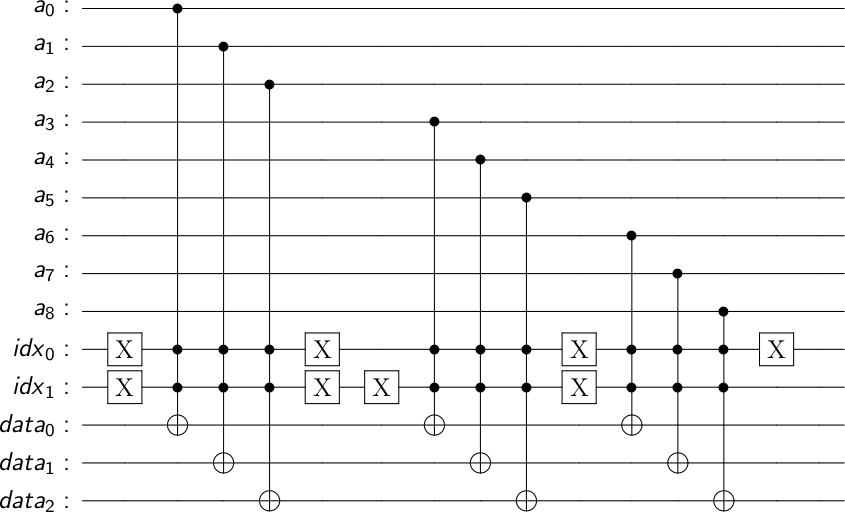
\includegraphics[scale=0.3]{results/indexer_3x3.png} 
  \caption{Indexer Circuit for a $3 \times 3$ matrix}
  \label{fig:indexer_circuit_3x3}
\end{figure*}

\begin{figure*}[!ht]
  \centering
  \begin{minipage}[b]{0.45\textwidth}
    \begin{equation*}
      A = \begin{bmatrix}%
        0 & 1 & 0 & 1 \\
        1 & 1 & 1 & 0 \\
        1 & 0 & 0 & 1 \\
        1 & 0 & 1 & 0 \\
      \end{bmatrix}
    \end{equation*}
  \end{minipage}

  \begin{subfigure}[b]{0.3\textwidth}
    \centering
    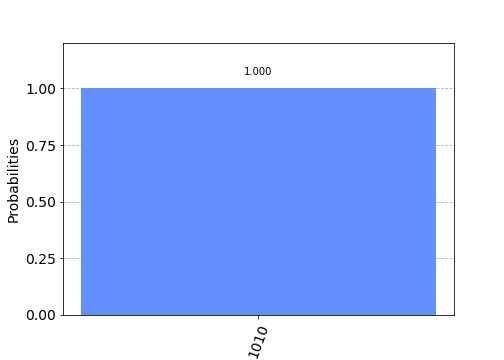
\includegraphics[width=\textwidth]{results/indexer_third_row.png} 
    \caption{Indexing the third row of $A$}
  \end{subfigure}
  %
  \begin{subfigure}[b]{0.3\textwidth}
    \centering
    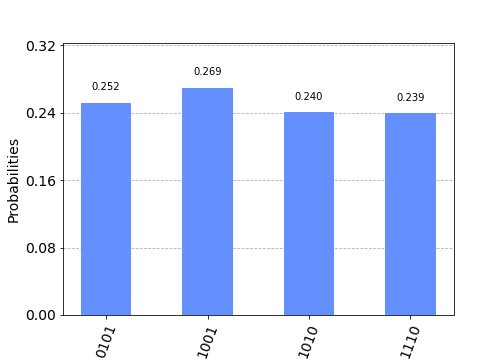
\includegraphics[width=\textwidth]{results/indexer_superposition.png} 
    \caption{Indexing $A$ using a superposition of the index}
  \end{subfigure}

  \caption{Indexer circuit functionality}
  \label{fig:indexer_func}
\end{figure*}

We report the gate counts, circuit depth, and number of qubits used when
targeting Aer simulator in Tables \ref{table:marking_oracle_stats} and
\ref{table:circuit_stats}. Further, we report transpilation times in Table
\ref{table:transpilation_stats}. The sub-circuits used in constructing the
QVMP marking oracle are summarized in figures
\ref{fig:indexer_circuit_3x3} and \ref{fig:inner_product_circuit_3x1}.
Figures \ref{fig:indexer_func} and \ref{fig:inner_product_func}
demonstrate the functionality of these auxiliary circuits. We show the
marking oracle circuit for a 4x4 matrix in Fig
\ref{fig:marking_oracle_4x4}.

\section{Analysis} \label{sec:analysis}

The QVMP oracle is a blackbox that checks if $(Ay - z)_i \neq 0$, where $A$,
$y$, $z$, and $i$ are as defined in the Alg \ref{alg:qvmp_grover}. Qiskit does
not offer automatic compilation of programming constructs like classical arrays to a
quantum circuit. The programmer has to define these operations on a per-problem
specific basis. The QVMP oracle is composed of the following two sub-circuits:
the indexer circuit and the inner product circuit.

\subsection{Indexer Circuit}


The role of the indexer is to output $A[i]$, where $A$ is an $m \times n$
matrix and $i$ is an integer index. We encode the matrix $A$ using
$size(A)$ qubits, where $size(A)$ is the total number of elements in $A$.
The integer index is encoded using $log_2(m)$ qubits in the binary format.

If we observe the functionality of the indexer closely, we see that
it is isomorphic to a multiplexer. In other words, the indexer
selects a specific row given a selector (which is the index in our
case). We can implement the indexing operation either as an in-place
(Fig \ref{fig:indexer_circuit_3x3}) or out-of-place operation
(\cite{roy_synthesis_2012}). The in-place solution requires more qubits, while
the out-of-place solution increases the circuit depth and is a little more
tricky to integrate with the rest of the oracle. For simplicity, we decided to
go with the in-place version.
      
Fig \ref{fig:indexer_func} shows the indexer circuit in action. When the index
qubits are not in a superposition state, we measure $A[i]$ with $100\%$
probability. On the other hand, if the index bits are in a superposition, we
measure multiple rows of $A$ depending on the superposition. The index
superposition lets us index multiple rows of $A$ at a time, but we can only
observe one of them when measured.

An interesting point to note is that unlike a classical multiplexer which
checks for the selector bits in parallel, the quantum indexer has to check
every index permutation sequentially. This pattern can be seen in the way
the $X$ gates are applied to the index qubits before applying the Tofolli
gate.

\subsection{Inner Product Circuit}

The inner product circuit \ref{fig:inner_product_circuit_3x1}, as the name
suggests, computes the inner product between two vectors encoded as qubits. Our
specific implementation only handles binary numbers (where multiplication is
defined as logical $AND$ and addition as logical $OR$), but can be easily
extended to support other data types.

% Inner Product
\begin{figure*}[!ht]
  \centering
  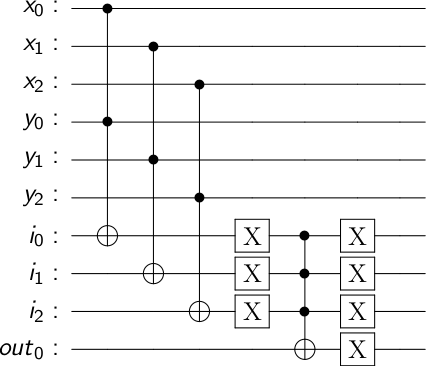
\includegraphics[scale=0.4]{results/inner_product_3x1.png} 
  \caption{Inner Product Circuit for $3 \times 1$ vectors}
  \label{fig:inner_product_circuit_3x1}
\end{figure*}
\begin{figure*}[!ht]
  \centering
  \begin{minipage}[b]{0.45\textwidth}
    \begin{align*}
      x = \begin{pmatrix}1\\1\\1\\1\end{pmatrix} \text{, } y = \begin{pmatrix}1\\0\\1\\0\end{pmatrix} \\
    \end{align*}
  \end{minipage}
  \begin{subfigure}[b]{0.3\textwidth}
    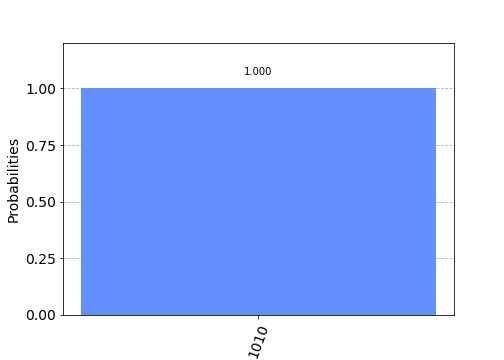
\includegraphics[width=\textwidth]{results/inner_product_true.png} 
    \caption{Inner product circuit outputting $1$}
    \label{fig:inner_product_example_true}
  \end{subfigure}

  \begin{minipage}[b]{0.45\textwidth}
    \begin{align*}
      x = \begin{pmatrix}0\\1\\0\\1\end{pmatrix} \text{, } y = \begin{pmatrix}1\\0\\1\\0\end{pmatrix} \\
    \end{align*}
  \end{minipage}
  \begin{subfigure}[b]{0.3\textwidth}
    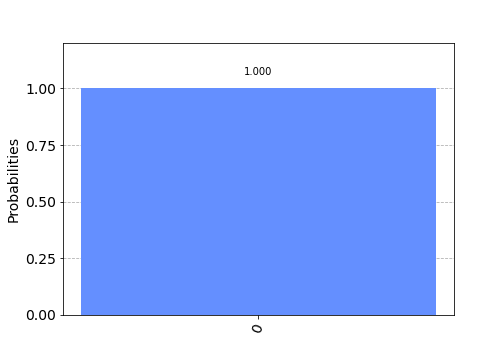
\includegraphics[width=\textwidth]{results/inner_product_false.png} 
    \caption{Inner product circuit outputting $0$}
    \label{fig:inner_product_example_false}
  \end{subfigure}

\caption{Inner product circuit functionality}
\label{fig:inner_product_func}
\end{figure*}

The $AND$ operation is done using a Toffoli gate.  The $OR$ gate is then
trivially implemented using De-Morgan's law. Both of these operations are
out-of-place.

\subsection{QVMP Oracle}
\begin{figure*}
  \centering
  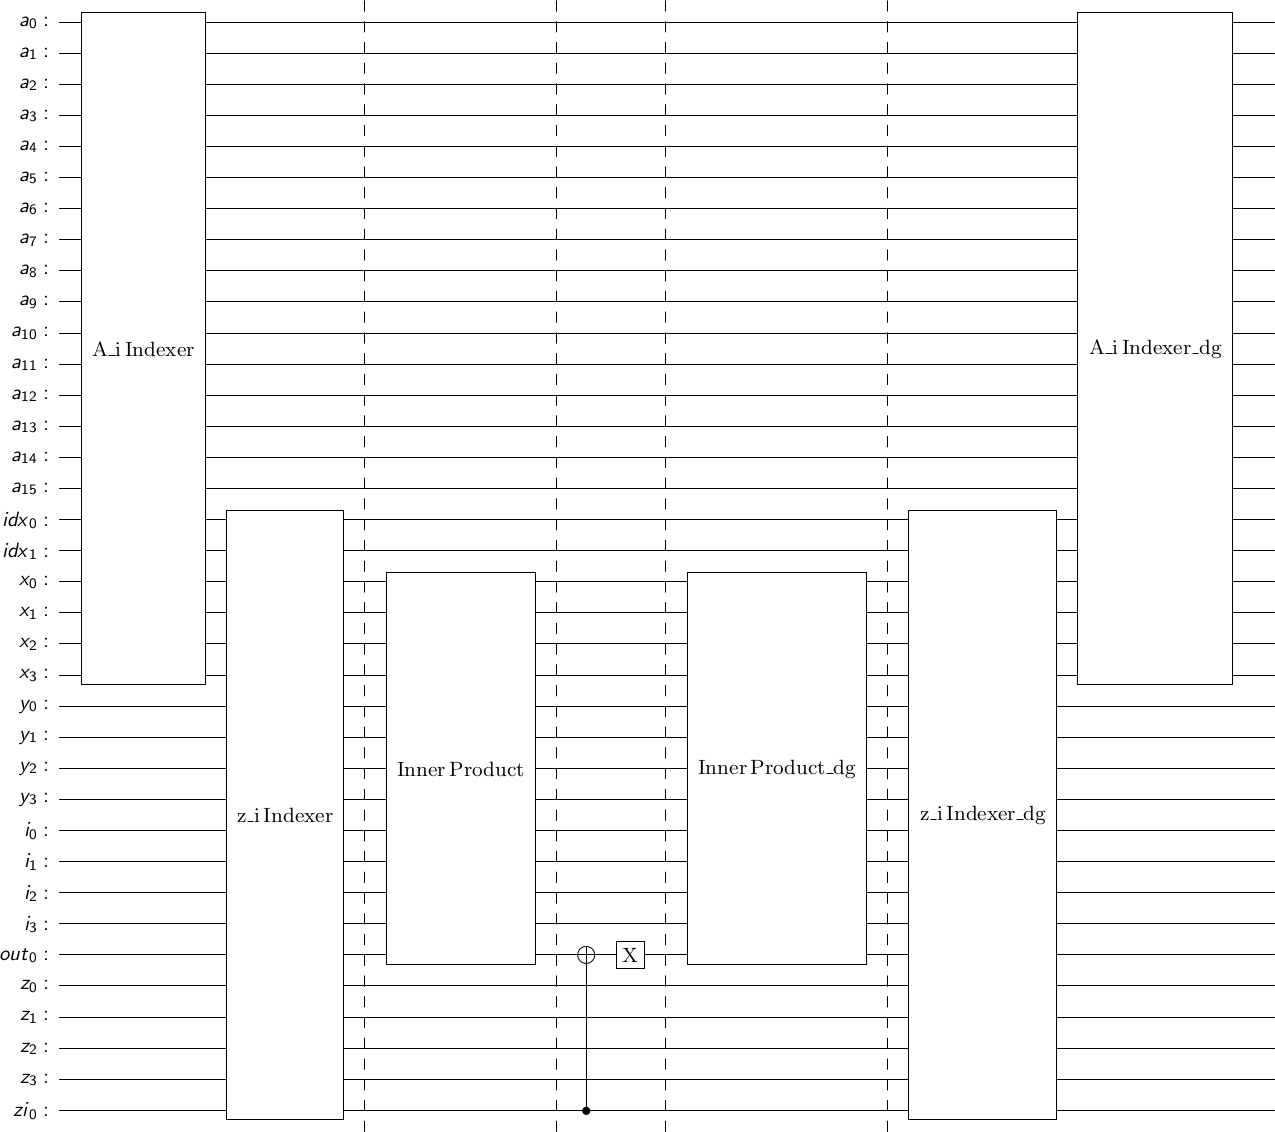
\includegraphics[scale=0.3]{results/oracle_circuit_4x4.png} 
  \caption{QVMP Marking Oracle for a $4 \times 4$ matrix}
  \label{fig:marking_oracle_4x4}
\end{figure*}
The marking oracle (Fig \ref{fig:marking_oracle_4x4}) is composed of both the
indexer and the inner product circuits. We first index into $A$ and $z$
outputting their results into ancilla qubits. Then we compute the inner product
$A_iy$. Finally, we compare the inner product with $z_i$. The comparator
circuit is a $CNOT$ with an additional $X$ gate applied to the target qubit.

As mentioned in Section \ref{sec:grover_oracles}, Grover's algorithm needs an
oracle which performs a phase-flip on correct solutions. We can easily convert
the marking oracle to a phase-flip oracle by simply sandwiching the marker
qubit with $XH$ and its inverse. This has the effect of putting the marker
qubit in the $\ket{-}$ state.

Another important point to note is that the oracle undoes the operations it
carries out in the workspace qubits. This is required so that the next
iteration of Grover can start with a clean workspace. Qiskit simplifies the
process of obtaining the inverse circuits. Every \verb|QuantumCircuit| object has
an inverse method which yields the corresponding circuit.

\vfill

\subsection{Overall Circuit}


\begin{table*}[t]
  \centering
  \begin{tabular}{|c||c|c|c|c|c||c|c|c|c|} 
   \hline
   Order & ccx & cx & mcx & mcxgray & x & Total Gates & Circuit Depth & Qubit Count \\
   \hline
   2 & 18 & 1 & 0 & 0 & 13 & 32 & 21 & 15 \\
    4 & 8 & 1 & 42 &  & 33 & 84 & 57 & 36 \\
    8 & 16 & 1 & 144 & 2 & 73 & 236 & 177 & 101 \\
    16 & 32 & 1 & 0 & 546 & 153 & 732 & 609 & 326 \\
    24 & 48 & 1 & 0 & 1202 & 235 & 1486 & 1297 & 679 \\
    32 & 64 & 1 & 0 & 2114 & 313 & 2492 & 2241 & 1159 \\
    64 & 128 & 1 & 0 & 8322 & 633 & 9084 & 8577 & 4360 \\
  \hline
  \end{tabular}
  \caption{VMP Marking Oracle Stats}
  \label{table:marking_oracle_stats}
\end{table*}

\begin{table*}[t]
  \centering
  \begin{tabular}{|c||c|c|c|c|c|c|c|c|c||c|c|c|} 
   \hline
   Order & ccx & cx & h & mcx & mcxgray & u1 & u2 & u3 & x & Total Gates & Circuit Depth & Qubit Count \\
   \hline
   2 &  72 & 4 & 13 &  & 4 & 9 & 116 & 2 & 49 & 269 & 94 & 15 \\
  4 &  56 & 7 & 33 & 294 & 7 & 15 & 495 & 5 & 219 & 1131 & 415 & 36 \\
  8 &  112 & 7 & 97 & 1008 & 21 & 15 & 1406 & 5 & 493 & 3164 & 1255 & 101 \\
  16 &  704 & 22 & 321 &  & 12034 & 45 & 14309 & 19 & 3286 & 30740 & 13445 & 326 \\
  24 &  1056 & 22 & 673 &  & 26466 & 45 & 29842 & 19 & 5070 & 63193 & 28581 & 679 \\
32 & 1728 & 27 & 1153 &  & 57105 & 55 & 62542 & 24 & 8326 & 130960 & 60564 & 1159 \\
      \hline
  \end{tabular}
  \caption{VMP Circuit Stats}
  \label{table:circuit_stats}
\end{table*}

\begin{table*}[!ht]
  \centering
  \begin{tabular}{|c|c|}
   \hline
    Order & Time (in seconds) \\
   \hline
    2 & 0.24860209489997942s \\
    4 & 0.8189974269000686s \\
    8 & 2.3804883372999486s \\ 
    16 & 27.484900246300004s \\
    24 & 66.20581728570009s \\
    \hline
  \end{tabular}
  \caption{VMP Circuit Transpilation Stats}
  \label{table:transpilation_stats}

\end{table*}

To complete the circuit, we need to apply Grover's search followed by amplitude
amplification. Qiskit provides the \verb|AmplificationProblem| routine which lets
you describe a search problem in the form of an oracle, initial state
preparation, and good states. We use this routine to build the necessary
circuits. For the Grover sub-circuit $G_i$, the state preparation is set to a
Hadamard on the objective qubits. For amplitude amplification, we pass $G_i$ as
the state preparation parameter.

Figures \ref{table:marking_oracle_stats} and \ref{table:circuit_stats} show metrics
associated with gate count, qubit count, and circuit depth for the oracle
transpilation and overall circuit transpilation respectively. After
transpilation, the Qiskit compiler decomposes higher-level gates to match the
gate set supported by the backend. We see that the qubit count rises to more
than 1000 for even small matrices of order 32. Further, transpilation onto the
Aer backend added gates that we not part of the high-level design (like $U_2$
and $U_3$). This results in a large increase in the number of quantum
operations performed. The transpilation time rises exponentially with an
increase in the order of the matrix (reaching slightly more than a minute for
an order 24 matrix), thereby slowing the development process.

\vfill

\subsection{Optimization Opportunities}

The implementation of the QVMP oracle can be further optimized. Note that the
matrix $A$ is not used for the rest of the oracle after the index operation.
This means that we can use $A$ as the oracle workspace to finish the rest of
the operations. Since quantum gates are reversible, we will be able to get back
$A$ by applying the reverse operations. This will reduce the number of qubits
required at the cost of increasing circuit depth.

\subsection{Challenges}

Implementing Grover oracles in Qiskit is cumbersome and error-prone. While the
library offers some routines for automating oracle synthesis, the tooling is
only limited to integers and boolean operators. This makes it challenging to
implement more complex oracles that have succinct classical descriptions.
Grover oracles typically try to emulate a classical operation, and the task of
implementing the oracle amounts to writing the equivalent quantum circuits. We
can develop tooling that takes a classical description of a Grover oracle and
automatically synthesize that into an quantum circuit. Qiskit offers the \verb|@classical_function|
decorator to do this, but as mentioned above, it is only
limited to integers. We believe that there is scope to extend the synthesis to
higher-level data types (like arrays and structs) and operators (like
indexing). This will boost developer productivity and make it easier to iterate
on quantum search problems.

Another challenge revolves around verification of correctness. Due to the
non-deterministic nature of quantum computing, it is more nuanced and
challenging to verify outputs. Simulators help alleviate this problem, but they
do not scale very well. For the QVMP case, as highlighted before, compilation
of a circuit for an order 32 square matrix is quite slow. Further, the Aer
simulator can only run circuits using less than 32 qubits. This inhibits the
practicality of algorithms like QVMP. 

As of this writing, NISQ machines support around 50-100 qubits. From Fig
\ref{table:circuit_stats}, this means that we are only able to run QVMP for
matrices of order 4 to 8.  The speedup of the quantum algorithm shows up on
matrices of much larger size.  Quantum noise makes it harder to put QVMP to
practical use. Our findings show that NISQ machines and simulators do not have
the resources to support solving a VMP problem of sufficient size.

\printbibliography[title=Bibliography]

\end{document}

%%% Local Variables:
%%% mode: latex
%%% TeX-master: t
%%% End:
